\documentclass{standalone}
\usepackage{pgfplots}

\begin{document}

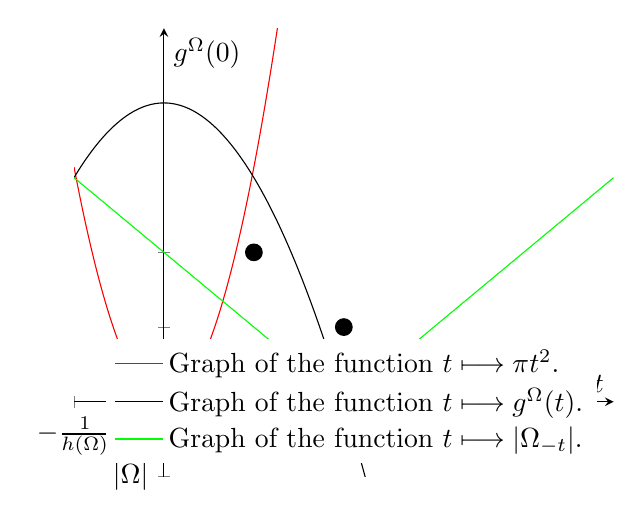
\begin{tikzpicture}
    \begin{axis}[
        axis lines=middle,
        xlabel=$t$,
        ylabel=$g^\Omega(0)$,
        xmin=-1, xmax=5,
        ymin=-1, ymax=5,
        xtick={-1, 0, 1, 2},
        ytick={-1, 0, 1, 2},
        xticklabels={$-\frac{1}{h(\Omega)}$, $0$, $\frac{1}{h(\Omega)}$, $r$},
        yticklabels={$|\Omega|$, $g^\Omega(0)$},
        legend pos=south east,
        legend cell align=left,
        legend style={draw=none},
        domain=-1:5,
        samples=100,
        smooth,
        every axis plot post/.append style={
            mark options={fill=black, mark size=3pt}
        }
    ]
        \addplot [red] {pi*x^2};
        \addlegendentry{Graph of the function $t \longmapsto \pi t^2$.}
        
        \addplot [black] {-x^2 + 4};
        \addlegendentry{Graph of the function $t \longmapsto g^\Omega(t)$.}
        
        \addplot [green] {abs(x - 2)};
        \addlegendentry{Graph of the function $t \longmapsto |\Omega_{-t}|$.}
        
        \addplot [mark=*, mark size=3pt] coordinates {(1, 2)};
        \addplot [mark=*, mark size=3pt] coordinates {(2, 1)};
    \end{axis}
\end{tikzpicture}

\end{document}